%%
%% Template intro.tex
%%

\chapter{Mapping the Night Sky}
\label{cha:astro}

When many people think about astronomy, the first things that pop into their mind are breathtaking
images of the sky like the famous Hubble Deep Field. But pretty images alone are not enough to do
real science. For us to make any meaningful observations about astronomical objects, we need actual
quantitative measurements. This chapter begins with an overview of spectroscopy and photometry, the
two most important tools in optical astronomy used to study the sky (Section \ref{sec:spec}).
We then look at important astronomical concepts like fluxes, magnitudes, colours, and the
equatorial coordinate system (Section \ref{sec:flux}, \ref{sec:mag}, and \ref{sec:map}). This will
give us a better understanding of the SDSS and the VST ATLAS datasets, which are introduced in
Section \ref{sec:datasets}. The chapter ends with a brief discussion on dust extinction, a
potential problem in the SDSS dataset that we shall need to take care of (Section \ref{sec:dust}).


\section{Spectroscopy and Photometry} \index{spectroscopy} \index{photometry}
\label{sec:spec}

Spectroscopy was born when Isaac Newton discovered in 1666 that white light can be split into a
rainbow by passing it through a glass prism. In modern-day astronomy, we use diffraction grating to
disperse light and measure the amount of electromagnetic radiation, or flux, emitted from a
celestial object at small wavelength intervals. As the name implies, we end up with a spectrum,
like the one shown in Figure \ref{fig:vega}. The shape of the spectrum and its absorption lines
allow us to deduce many useful properties about the object such as its temperature and chemical
composition.

Unfortunately, it can be very difficult to take high resolution spectra of faint objects since we
are spreading light thinly across many wavelengths. Photometry gets around this problem by
separating light into fewer groups and thus reducing the wavelength resolution \cite[Chapter
1]{romanishin02}. Specifically we have a set of filters, each of which can be put in front of the
CCD camera to allow only light from certain wavelengths to pass through. Associated with each
filter is a transmission function $T(\lambda)$ that tells us the fraction of light that the filter
will transmit at wavelength $\lambda$. Figure \ref{fig:vega} shows $T(\lambda)$ of the five
bandpasses (u, g, r, i, and z) that are used in the SDSS.

\begin{figure}[tbp]
	\centering 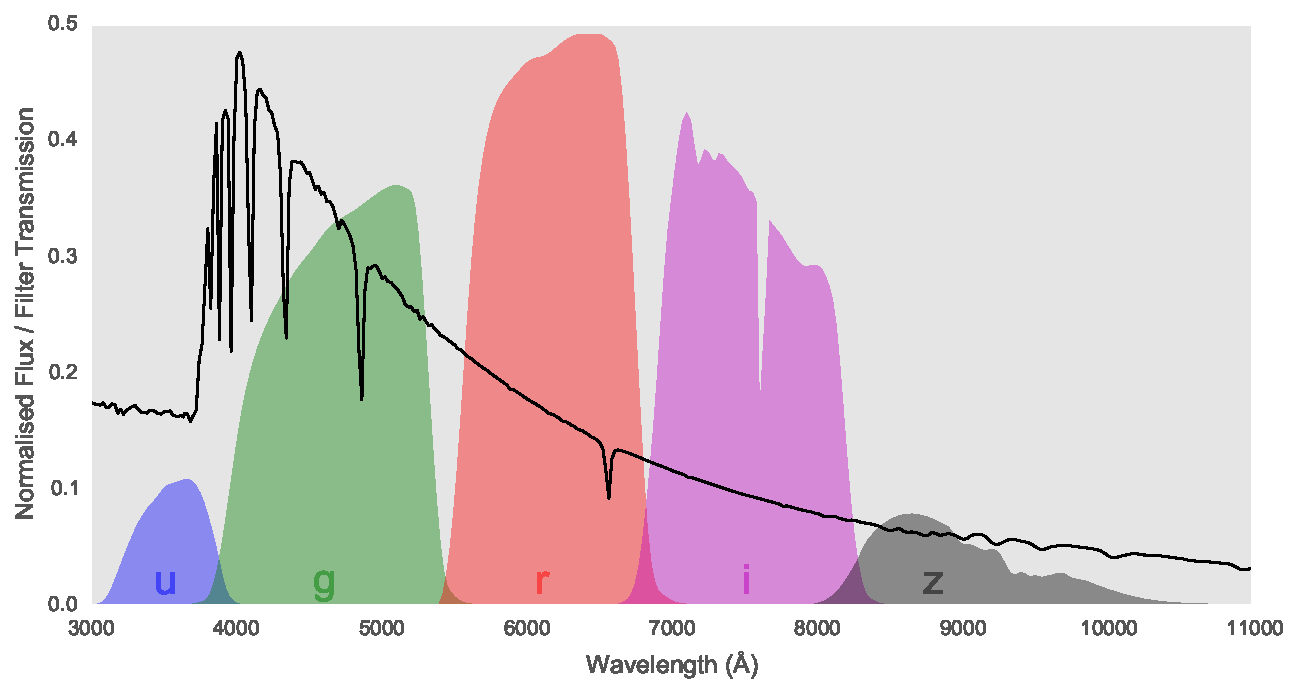
\includegraphics[width=\textwidth]{figures/2_astro/vega_filters_and_spectrum}
	\caption[Spectrum of the star Vega and the ugriz bandpasses]{The black curve is the
		spectrum of Vega, the fifth brightest star in the night sky. The spectrum tells us how
		much radiation Vega emits at each wavelength. We also show five transmission functions,
		one for each of the five ugriz filters. The transmission function tells us how much light
		can get through the filter at each wavelength.} \label{fig:vega} \index{Vega}
\end{figure}


\section{Measuring Fluxes} \index{flux}
\label{sec:flux}

When light hits the CCD, all we have initially are counts of photons, one for each pixel.
The first challenge is to assign the photons to distinct objects. Two models are used
in the SDSS, depending on whether we assume the object is an extended source or a point source.


\subsection{Petrosian Flux} \index{flux!Petrosian}
\label{sub:petrosian}

Galaxies are extended-source objects so we need to define an aperture radius, within which
all the photons are added together to obtain the flux of the galaxy. Since galaxies have
poorly defined edges, a consistent method to pick the aperture radius is required.
\shortciteN{blanton01} define a quantity called the Petrosian ratio:
	\begin{IEEEeqnarray*}{lCl}
		\mathfrak{R}_p(r) = \frac{\int_{0.8r}^{1.25r} 2\pi s I(s) \, ds}{\pi (1.25^2 - 0.8^2) r^2}
							\bigg/ \frac{\int_0^r 2\pi s I(s) \, ds}{\pi r^2}
	\end{IEEEeqnarray*}
This is the ratio of the mean local surface brightness over an annulus at $r$ to the mean
surface brightness within $r$. The quantity $I(r)$ is the galaxy surface brightness profile
and can be estimated from the photon count. With this, we define the Petrosian
radius $r_p$ as the radius such that $\mathfrak{R}_p(r_p) = 0.2$. This is one of the features
in the SDSS dataset that will prove to be very useful in distinguishing galaxies from
point-source objects. The aperture radius is then chosen to be $2r_p$ to ensure that almost
all of the light from a typical galaxy is captured. Finally for each bandpass, we can calculate
the corresponding Petrosian flux as
	\begin{IEEEeqnarray*}{lCl}
		f &=& \int_{0}^{2 r_p} 2 \pi s I(s) \, ds
	\end{IEEEeqnarray*}

\subsection{Point Spread Function Fitting} \index{flux!PSF}
\label{sub:psf}

Stars, quasars, and white dwarfs are unresolved point sources so they can be modelled by a point
spread function (PSF). This approach is particularly useful when we examine a dense region like a
globular cluster. In such places, given the amount of overlap, it would be very difficult define an
aperture that includes only photons from an object and excludes all others from the neighbours. In
PSF fitting, we assume that all objects have the same shape, which allows us to fit a Gaussian model
to each of them. We then iteratively vary the position and flux of the objects until the model
produces the observed light distribution \cite[Chapter 10]{palmer01}. The flux estimated by the
converged model is called the PSF flux.

\section{Magnitudes and Colours} \index{magnitude}
\label{sec:mag}

\subsection{Apparent Magnitudes} \index{magnitude!apparent}
\label{sub:apparent}

The fluxes of the brightest and the dimmest objects in the sky can differ by many orders of
magnitudes. This motivates us to take one step further and convert fluxes to inverse hyperbolic sine
(or arsinh) apparent magnitudes:
	\begin{IEEEeqnarray*}{lCl}
		m &=& -\frac{2.5}{\ln(10)} \Bigg[ \arsinh\bigg(\frac{f/f_0}{2b}\bigg) + \ln(a) \Bigg]
	\end{IEEEeqnarray*}
where $f_0$ is the flux of the object with a conventional magnitude of 0 and $a$ is the softening
parameter. A nice feature of this magnitude system is that for bright objects with a high
signal-to-noise ratio, it behaves like a logarithmic scale, i.e. with every decrease of 1 in the
magnitude scale, the object becomes 2.5 times brighter.\footnote{ The reader might wonder why the
	scale works in reverse, with a small magnitude corresponding to more brightness. This is the
	convention created two millennia ago by the Greek astronomer Hipparchus, which, for better or worse,
	has stuck with us ever since.} At the same time, as the flux tends toward zero for fainter objects,
the arsinh function (unlike the log function) ensures that the magnitudes are still well-defined
\cite{lupton99}.

\subsection{Absolute Magnitudes and Colours} \index{magnitude!absolute} \index{colour}
\label{sub:colours}

The problem with apparent magnitudes is their dependence on distance. Objects that are further away
from us are fainter and hence have higher apparent magnitudes. Of course, being further away does
not change anything fundamental about an object like whether it is a star or a galaxy. Thus if we
want to study their intrinsic properties, we need to remove this dependency. One method is to
convert to the absolute magnitude, which is defined as the object's apparent magnitude if it were
exactly 10 parsecs away from Earth:
	\begin{IEEEeqnarray*}{lCl}
		M &=& m - 5 \log_{10} \bigg(\frac{D}{10}\bigg)
	\end{IEEEeqnarray*}
This conversion requires the knowledge of $D$, the actual distance of an object in parsecs. In
practice, it is often difficult to estimate $D$, so we resort to an easier method of taking the
difference between the amount of light received in two bandpasses. For example, the $u -g$ colour is
calculated as
	\begin{IEEEeqnarray*}{lCl}
		m_{u-g} &=& m_u - m_g \\
		        &=& M_u + 5 \log_{10} \bigg(\frac{D}{10}\bigg) -
		            M_g + 5 \log_{10} \bigg(\frac{D}{10}\bigg) \\
		        &=& M_u - M_g
	\end{IEEEeqnarray*}
Note that the conversion factor disappears and the colour does not change with distance. In
addition, the difference between two magnitudes depends on the average slope of the spectrum. Thus
colours measure the general shape of an object's spectrum, which in turn can reveal many useful
properties such as a star's temperature.


\section{Equatorial Coordinate System} \index{equatorial coordinate system}
\label{sec:map}

Imagine a very large celestial sphere \index{celestial sphere} with Earth at its centre. By
projecting onto the inside surface of this sphere, we have a way to specify the position of any
astronomical object. In this thesis, we use the equatorial coordinate system, where an object's
position is specified by two numbers, a right ascension \index{right ascension} (ra) and a
declination \index{declination} (dec). Figure \ref{fig:mollweide} shows the Mollweide projection of
the celestial sphere. We shall use this map throughout the thesis to visualise some results.

\begin{figure}[tbp]
	\centering
	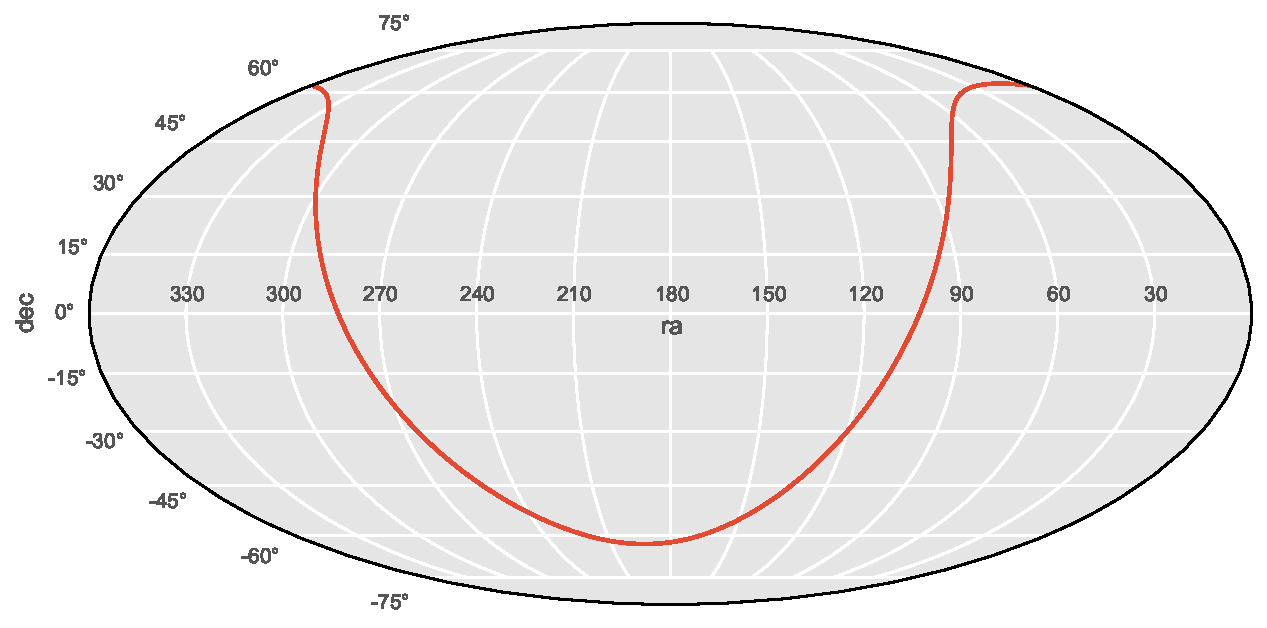
\includegraphics[width=\textwidth]{figures/2_astro/mollweide_map}
	\caption[Mollweide projection of the celestial sphere]{This is the Mollweide projection
		of the celestial sphere under the equatorial coordinate system.
		The red line indicates the plane of the Milky Way. To avoid cluttering, the coordinate labels will not be shown on later maps.}
	\label{fig:mollweide} \index{Mollweide projection}
\end{figure}

The equatorial coordinate system, like any other systems, needs to have a reference point. Here
anything on the celestial sphere that is directly above the Earth's equator will have a declination
of 0\deg. To define a zero point for the right ascension, we use the fact that the centre of the
Sun passes through the plane of the Earth's equator twice a year. The first crossing point usually
happens on 21 March and is called the vernal equinox\index{vernal equinox}. We now define the right
ascension of the vernal equinox to be 0\deg~\cite[Chapter~1]{sparke07}.\footnote{ There is actually
    a slight complication. Since the Earth's rotation axis is not fixed due to
    precession\index{precession}, the ra-dec coordinates of an object relative to the origin will
    actually change slowly over time. Thus we need to also fix a time in which the coordinates are
    measured. In many surveys like the SDSS, 1 January 2000 12:00 Terrestrial Time is chosen as a
    reference point.}




\section{Datasets}
\label{sec:datasets}

We now have all the required background to understand the features in the two datasets used in our
experiments. Below we give a quick overview of what each dataset contains. For more information on
how to obtain them, refer to Appendix \ref{cha:datasets}.

\subsection{SDSS Dataset} \index{SDSS}
\label{sub:sdss}

\begin{figure}[p]
	\centering
	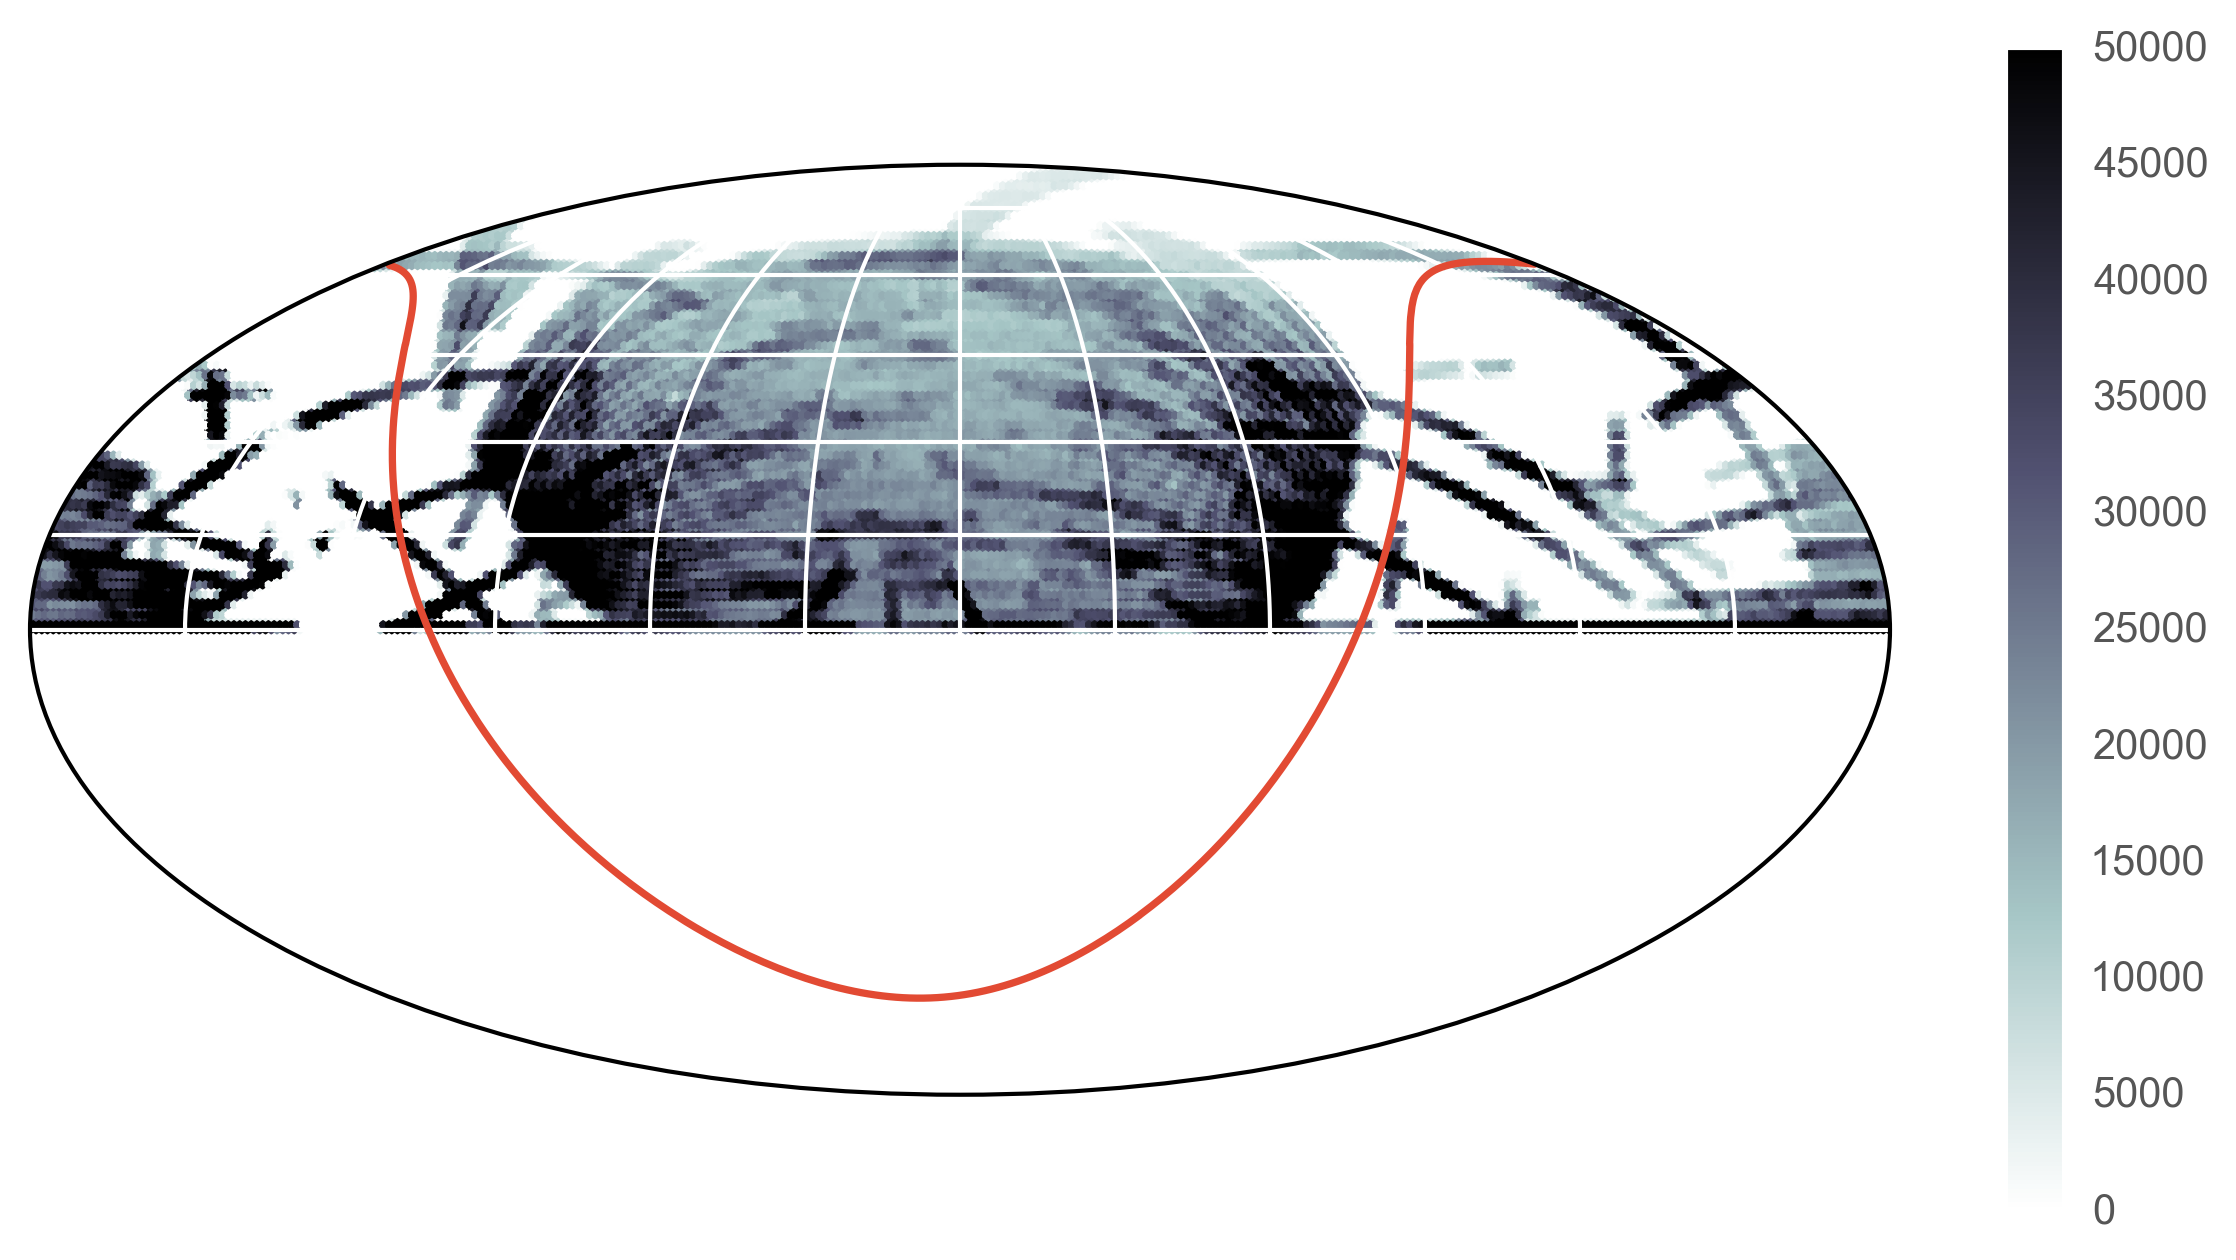
\includegraphics[width=\textwidth]{figures/4_expt1/map_prediction_forest_all}
	\caption[Coverage of the SDSS]{The distribution of the 800 million scanned objects
		in the SDSS: Note that the coverage is not uniform. A darker colour
		corresponds to more objects being scanned in a particular area. The unit
        of the colourbar is the object count in a hexagon.}
	\label{fig:coverage}
\end{figure}

\begin{figure}[p]
    \centering
    \begin{subfigure}{.5\textwidth}
        \centering
        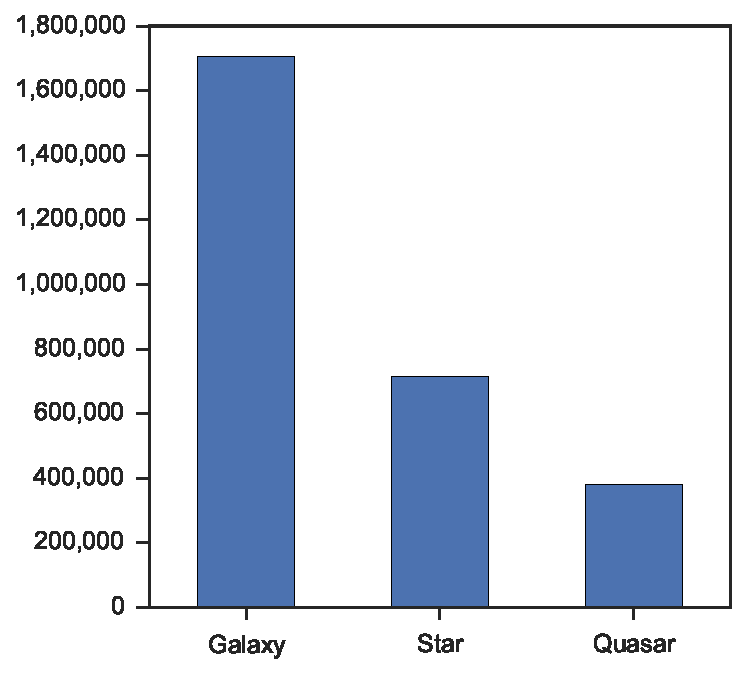
\includegraphics[width=0.99\textwidth]{figures/2_astro/sdss_class_distribution}
        \caption{SDSS Dataset}
        \label{fig:class_dist_sdss}
    \end{subfigure}%
    \begin{subfigure}{.5\textwidth}
        \centering
        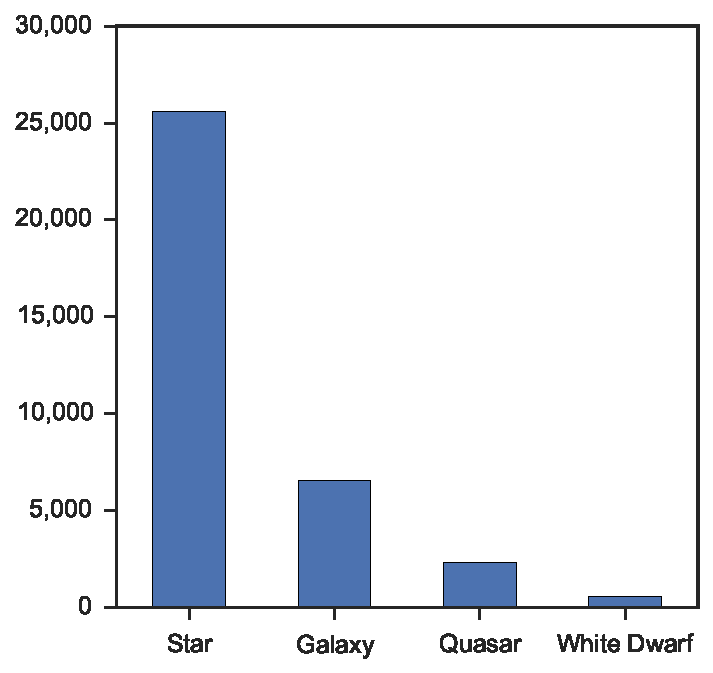
\includegraphics[width=0.99\linewidth]{figures/2_astro/vstatlas_class_distribution}
        \caption{VST ATLAS Dataset}
        \label{fig:class_dist_vst}
    \end{subfigure}
    \caption[Distribution of the classes in the SDSS and VST ATLAS datasets]{
        Class distribution of the labelled objects in the SDSS and VST ATLAS datasets: Observe
        that both datasets exhibit the problem of class imbalance. Most objects in the
        SDSS dataset are galaxies, while stars are the dominant class in the VST ATLAS dataset.}
    \label{fig:class_dist}
\end{figure}

The main dataset in our investigation comes from the SDSS, a comprehensive survey of the Northern
Sky that began operation in 2000. This dataset consists of 800 million objects, covering 14,055
square degrees, or about a third of the celestial sphere \cite{alam15}. Figure \ref{fig:coverage}
shows the coverage of the survey. For each object, we are given 11 features:
	\begin{itemize}
		\item The PSF magnitude in each of the five ugriz bands.
		\item The Petrosian magnitude in each of the five ugriz bands.
		\item The Petrosian radius in the r-band.
	\end{itemize}
Only 2.8 million out of the 800 million objects have been spectroscopically classified into three
classes: galaxies, quasars, and stars. From Figure \ref{fig:class_dist_sdss}, we can see that the
number of galaxies is twice that of stars and four times that of quasars. This leads to the
problem of class imbalance. In Chapter \ref{cha:ml} we shall discuss some approaches to minimise
the bias toward the dominant class during classification. Also note that both the labelled and the
unlabelled sets are not random samples of the sky. For example, since astronomers are particularly
interested in studying quasars, these objects are over-represented in the collection.




\subsection{VST ATLAS Dataset} \index{VST ATLAS}
\label{sub:vstatlas}

A second and much smaller dataset comes from a more recent survey, the VST ATLAS. This project aims
to survey 4500 square degrees of the Southern Sky to roughly the same depth as the SDSS
\cite{shanks15}. There are about 35,000 objects in total which have been classified by experts into four
classes: stars, galaxies, quasars, and white dwarfs. For each object, we are provided with 7
features:
	\begin{itemize}
		\item The calibrated magnitude from the r-band.
		\item Four colour indices using the ugriz filters: $u-g$, $g-r$, $r-i$, and $i-z$.
		\item Two colour indices in the infrared: $r-W1$ and $W1-W2$.
	\end{itemize}
The two infrared channels $W1$ and $W2$ are measured by the Wide-field Infrared Survey Explorer
(WISE), one of NASA's space telescopes. These channels will prove useful in distinguishing
between classes. As we can see from Figure \ref{fig:class_dist_vst}, the problem of class
imbalance is even worse in this dataset. For instance, we have 43 times more stars than white
dwarfs. Since research is still on-going, the coordinates of the objects are not yet publicly
available.



\section{Dust Extinction} \index{dust extinction} \index{reddening correction}
\label{sec:dust}

As light travels from its source to us, it can be absorbed and scattered by interstellar dust. The
scattering is especially strong at shorter wavelengths. This means that less of the blue light
arrives on Earth and the object will appear redder than it actually is.

This would not be a big problem if the reddening process were uniform throughout the
celestial sphere, since all the magnitudes and colours will simply shift by a constant
term. Indeed, this is the case with the VST ATLAS, since the field where the objects were
surveyed exhibits no drift in the reddening.
However, the SDSS covers a much larger portion of the sky. As shown in
Figure \ref{fig:reddening}, the reddening varies by quite a bit throughout the field. The
effect is particularly strong in the Milky Way region. Thus we might need to correct the SDSS
magnitudes for dust extinction.

\begin{figure}[tbp]
	\centering
	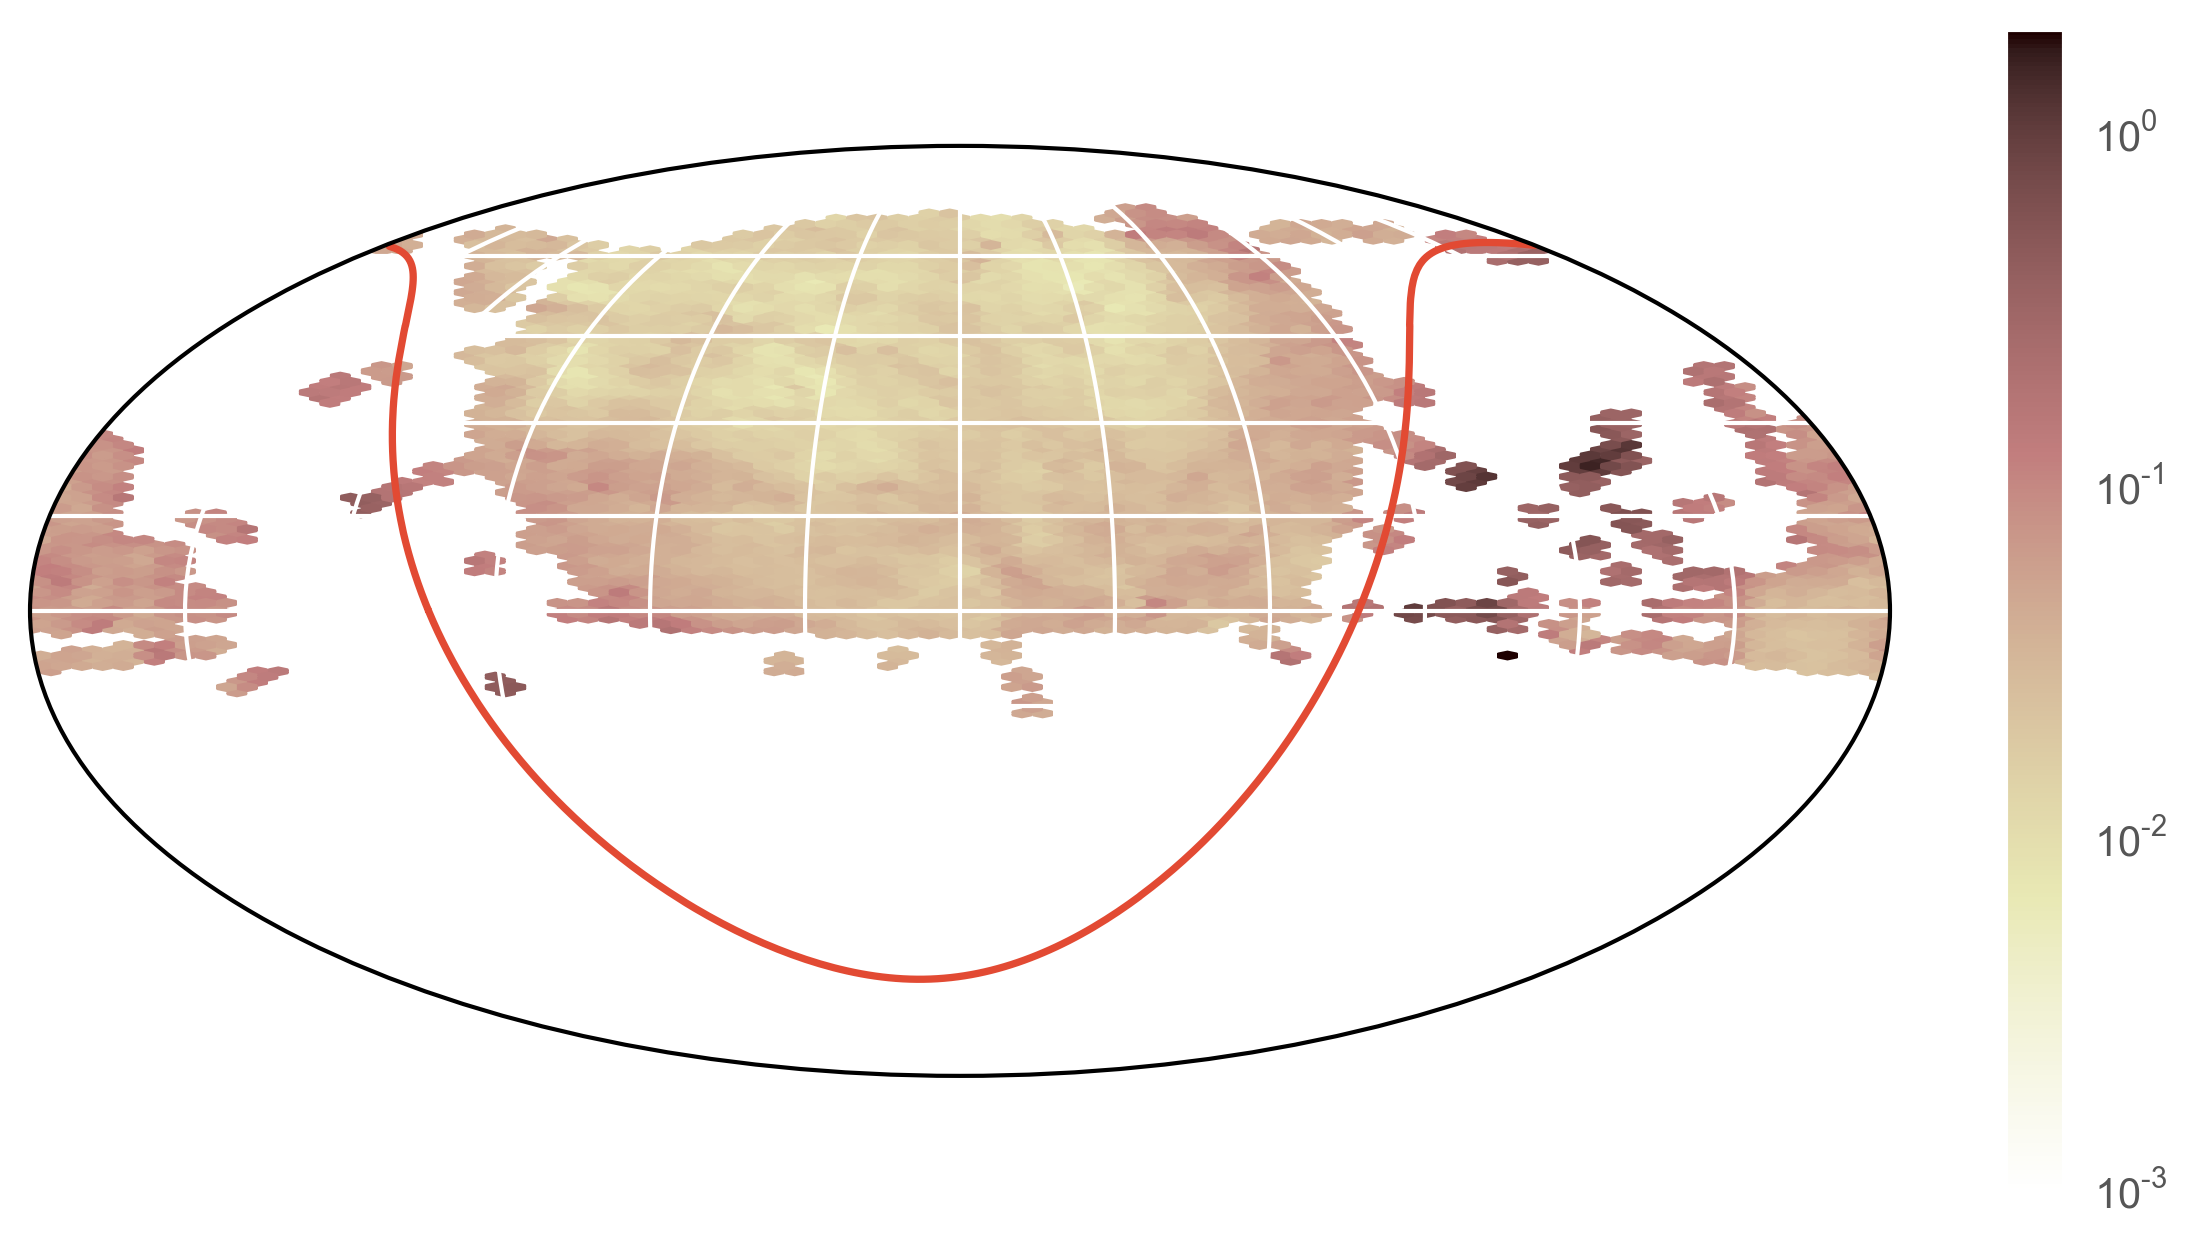
\includegraphics[width=\textwidth]{figures/2_astro/ebv_map}
	\caption[Galactic reddening map in the SDSS]{Galactic reddening $E_{B-V}$ map in the SDSS:
		A darker colour indicates a greater amount of reddening.}
	\label{fig:reddening}
\end{figure}

Three competing extinction vectors currently exist in the literature. The most popular one for a
long time was created by \citeN{schlegel98}, who used the colours of nearby elliptical galaxies for
calibration. Later, \citeN{schlafly11} made some improvement with new data from the SDSS. Recently,
\citeN{wolf14} investigated quasars in the SDSS and found evidence of non-linearity in the
reddening map. For convenience, let us call the extinction vectors resulted from the above works
SFD98, SF11, and W14, after the authors' initials and year of publication. One interesting
question, which we shall explore in Chapter \ref{cha:expt1}, is whether applying any of these
vectors to the measurements will have any noticeable effect on the performance of the classifiers.



%%% Local Variables: 
%%% mode: latex
%%% TeX-master: "thesis"
%%% End: 
